\chapter{Knowledge-driven Acoustic Echo Retrieval \& \acs{BLASTER}}\label{ch:blaster}

\marginpar{%
    \footnotesize
    \textbf{Keywords:} Blind Channel Identification, Super Resolution, Sparsity, Acoustic Impulse Response.
    \\\textbf{Resources:}
    \begin{itemize}
        \item \href{https://doi.org/10.1109/ICASSP40776.2020.9054647}{Paper}
        \item \href{https://gitlab.inria.fr/panama-team/blaster}{Code}
        \item \href{https://hal.archives-ouvertes.fr/hal-02469901}{Open-access paper with supplementary material}
        \item \href{https://sigport.org/documents/blaster-grid-method-blind-and-regularized-acoustic-echoes-retrieval}{Slides}
        \item \href{https://youtu.be/rPaqZJIfpKo}{Presentation}
    \end{itemize}
}
\newthought{Synopsis} \synopsisChBlaster

\mynewline
The material presented in this chapter was previously published in~\cite{di2020blaster} and results from a collaboration with a colleague whose
domain of expertise is in the \CDdef/ framework.
The \CD/ framework applied for \AER/ is extracted from the related publication and briefly commented, while more attention is paid in grasping the motivation behind it.
Finally, this chapter recall the main findings of the paper bringing additional insight in the existing models for \AER/.

\section{Introduction}
\label{sec:blaster:intro}
% %Striking introducing sentence
% As deeply discussed so far, the temporal structure of the \RIRdef/ plays a central role in room acoustics and audio signal processing.
% % First echo is noise
% It is the result of multiple (indirect) sound propagation paths due to specular and diffuse reflections on the room's surfaces, leading to reverberation~\citeonly{Wang2011}.
% In such conditions, the perceived sound quality is often considered degraded and it is common to observe a detrimental decrease of performance as reverberation increases for applications such as speech recognition~\citeonly{Yoshoka2012} or music information retrieval~\citeonly{Barthet2010}.
% % or music virtual reality~\citeonly{DeMan2017}. %to observe a detrimental decrease of performances with reverberation. as well as music virtual reality~\citeonly{DeMan2017}.

% % Second echo is information
% On the other hand, RIRs contain very rich geometrical information about the acoustic scene.
% %which is independent from the source signal itself.
% %In contrast with well-consolidated methods,
% Recent \textit{echo-aware} works have shown that the knowledge of the timing of early reflections may boost performance in many audio signal processing applications,
% from dereverberation~\citeonly{Wu2006,Lin2008} to sound localization~\citeonly{Ribeiro2010,DiCarlo2019} and separation~\citeonly{Dokmanic2015a, Scheibler2017}.
% Moreover, it allows joint estimation of the receivers' positions~\citeonly{Salvati2016}, the reflective surfaces~\citeonly{Antonacci2012} and consequently the geometry of the room~\citeonly{Dokmanic2013, Crocco2017}.
% % or acoustic impedance of surfaces~\citeonly{Antonello2014, Bertin2016}.
% % beamforming \citeonly{Dockmanic2015},
% % such as for speech enhancement \citeonly{Wu2006}, source localization \citeonly{Ribeiro2010}, source separation \citeonly{Scheibler2017} and dereverberation \citeonly{Lin2009}
% % which are common pre-processing steps for many applications \citeonly{Gannot2017}

\AERdef/ consists in estimating the properties of the early (strong) acoustic reflections only in multi-path environments, and sometimes referred to as time delay estimation~\citeonly{chen2006time}.
To achieve this, several methods rely on a known source signal~\citeonly{park2017compressive,jensen2019method}.
In contrast, when multiple receivers attend an unknown single source, \AER/ can be seen as an instance of \SIMOdef/ \BCEdef/ problem, \ie/ estimating the filters entailing an unknown input observed output of a system.
A common approach for solving \AER/ in the context of \SIMO/-\BCE/ is to first blindly estimate a discrete version of the acoustic channels using the so-called cross-relation identity~\citeonly{xu1995least, crocco2016estimation}.
The location of the echoes are then chosen among the strongest peaks with ad-hoc peak-picking techniques.
Such methods are generally \emph{on-grid} in the sense that the estimation relies on a fixed grid of points and \textit{a priori} chosen filter lengths.
However, in practice, the true timings of echoes rarely match the sampling grid, thus leading to pathological issues called basis-mismatch in the field of compressed sensing.
To circumvent this issue, the authors of~\citeonly{tukuljac2018mulan} proposed to leverage the framework of finite-rate-of-innovation sampling to make one step towards off-grid approaches.
Despite promising results in the absence of noise and with synthetic data, the quality of the estimation highly relies on an initialization point.

\mynewline
Of particular interest in this paper is the recently proposed framework of \CDdef/~\citeonly{candes2014towards}.
By formulating an inverse problem as the recovery of a discrete measure over some parameter space, \CD/ has allowed to overcome imaging device limitations in many applications such as super-resolution~\citeonly{candes2014towards} or PALM/STORM imaging~\citeonly{denoyelle2019sliding}.
In this work, we formulate the problem of \AER/ for stereophonic mixtures, \ie/ using only microphone pairs, within the framework of continuous dictionaries.
The resulting optimization problem is convex and thus not prone to spurious minimizers.
The proposed method is coined \emph{\BLASTERdef/} and requires no parameter tuning.
The method is compared to state-of-the art on-grid approaches under various noise and reverberation levels using simulated data.


\section{Background in Acoustic Echo Estimation}\label{sec:blaster:background}

\subsection{Signal and measurement model}
We consider here the common setup of stereophonic mixtures, that is 2-channel microphone recordings.
% Consider the common setup where a band-limited and square-integrable source signal $\tilde{\src}$ is emitted.
% Due to the geometry of the room, the latter signal is both reflected (several times) and attenuated before reaching a set of two microphones.
Using the notation presented~\cref{ch:processing}, recorded signal at microphone $\idxMic\in\{1,2\}$ reads
\begin{equation}
    \label{eq:blaster:recordedSignal}
    \tilde{\mic}_i = \tilde{\src} \convCont \tilde{\flt}_i^\star + \tilde{u}_i
\end{equation}
where $\convCont$ denotes the (continuous) convolution operator, $\tilde{n}_i$ models some additive noise in the measurement process and $\tilde{\flt}_i^\star$ denotes the \RIRdef/.
In the remainder of this chapter, the superscript $\star$ refers to the ground truth.
Assuming the echo model, the \RIRs/ read
\begin{equation}
    \label{eq:blaster:def_filter_star}
    \tilde{\flt}^\star(t) = \sum_{\idxEch=0}^{\numEchs_i} \alpha_i^{(r)} \delta(t - \tau_i^{(r)})
\end{equation}
where $\numEchs_i$ is the (unknown) number of echoes.
\\In the noiseless case, that is when $\tilde{u}_i = 0$ for $i\in\{1,2\}$, we have the cross-relation identity
\begin{equation} \label{eq:blaster:cross-relation}
    \tilde{\mic}_1 \convCont \tilde{\flt}_2^\star = \tilde{\mic}_2 \convCont \tilde{\flt}_1^\star
\end{equation}
by commutativity of the convolution operator.

However, in practice, only sampled versions of the two recorded signals are available.
More precisely, we consider the measurement model introduced in~\cref{ch:processing}:
the incoming signal undergoes a (ideal) low-pass filter $\lowpassfilter$ with frequency support $\kintervcc{\sfrac{-\Fs}{2}}{\sfrac{\Fs}{2}}$ before being regularly sampled at the rate $\Fs$.
We denote $\disRecordedSignal_1,\disRecordedSignal_2\in\bbR^{2N}$ the two vectors of $2N$ (consecutive) samples and $i\in\{1, 2\}$ by
\begin{equation}
    \label{eq:blaster:measurement-process}
    \disRecordedSignal_i[n] =
    \kparen{\idealLowPassFilter \convDis \contRecordedSignal}\kparen{\frac{n}{\Fs}}
    \qquad
    \forall n \in\{0, \dots, 2N-1\}
    .
\end{equation}
%Let $\disRecordedSignal_1,\disRecordedSignal_2\in\kR^N$ denote the two vectors of $N$ consecutive samples that are such that $\disRecordedSignal_i[\ell] = \contRecordedSignal_i(\sfrac{\ell}{F_s})$ for $\ell\in\{1...N\}$, $i\in\{1, 2\}$ and  where $F_s$ is the sampling frequency.



%We denote $\disRecordedSignal\in\kR^N$ the $N$ consecutive samples, \ie/, such that $\disRecordedSignal[\ell] = \contRecordedSignal(\sfrac{\ell}{F_s})$ where $F_s$ is the sampling frequency.
% These $N$ consecutive samples will be denoted  $\disRecordedSignal\in\kR^N$ and satifies $\disRecordedSignal[\ell] = \contRecordedSignal(\sfrac{\ell}{F_s})$ $\forall\ell\in\{1...N\}$ where $F_s$ is the sampling frequency.

%the signals are notaccessible.  They are measured by sensors and discretized to be stored in a computer’s memory.


\subsection{Existing works}\label{subsec:blaster:sota}
Starting from the identity \cref{eq:blaster:cross-relation}, the common \SIMO/-\BCE/ cross-relation framework aims to compute $\contFilter_1, \contFilter_2$ solving the following problem in the discrete-time domain~\citeonly{lin2008blind}:
\begin{equation}
    \label{eq:blaster:xrel_toepl}
    \disFilterHat_1, \disFilterHat_2
    =
    \kargmin_{\disFilter_1, \disFilter_2}
    \;
    \tfrac{1}{2}
    \kvvbar{
        \scrT(\disRecordedSignal_1) \disFilter_2
        -
        \scrT(\disRecordedSignal_2) \disFilter_1
    }_2^2
    +
    \lambda
    \kvvbar{
        \disFilter
    }_1
\end{equation}
where $\disRecordedSignal_i$ and $\disFilter_i$ are the discrete, sampled version of $\contRecordedSignal_i, \contFilter_i$ respectively.
\\$\scrT(\disRecordedSignal_i)$ is the $(2N+L-1) \times L$ Toeplitz matrix (build as shown is~\cref{fig:blaster:toeplitz})
\marginpar{
    \centering
    \resizebox{\linewidth}{!}{
        

\tikzset{every picture/.style={line width=0.75pt}} %set default line width to 0.75pt

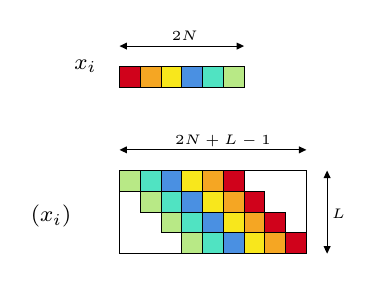
\begin{tikzpicture}[x=0.75pt,y=0.75pt,yscale=-1,xscale=1]
%uncomment if require: \path (0,300); %set diagram left start at 0, and has height of 300

%Shape: Rectangle [id:dp9681290386895156]
\draw   (190,80) -- (280,80) -- (280,120) -- (190,120) -- cycle ;
%Shape: Rectangle [id:dp4105274901835]
\draw  [fill={rgb, 255:red, 208; green, 2; blue, 27 }  ,fill opacity=1 ] (190,30) -- (200,30) -- (200,40) -- (190,40) -- cycle ;
%Shape: Rectangle [id:dp07108913371302106]
\draw  [fill={rgb, 255:red, 245; green, 166; blue, 35 }  ,fill opacity=1 ] (200,30) -- (210,30) -- (210,40) -- (200,40) -- cycle ;
%Shape: Rectangle [id:dp27992457661326675]
\draw  [fill={rgb, 255:red, 248; green, 231; blue, 28 }  ,fill opacity=1 ] (210,30) -- (220,30) -- (220,40) -- (210,40) -- cycle ;
%Shape: Rectangle [id:dp22621399339540804]
\draw  [fill={rgb, 255:red, 74; green, 144; blue, 226 }  ,fill opacity=1 ] (220,30) -- (230,30) -- (230,40) -- (220,40) -- cycle ;
%Shape: Rectangle [id:dp8143232980428775]
\draw  [fill={rgb, 255:red, 80; green, 227; blue, 194 }  ,fill opacity=1 ] (230,30) -- (240,30) -- (240,40) -- (230,40) -- cycle ;
%Shape: Rectangle [id:dp3194122969586535]
\draw  [fill={rgb, 255:red, 184; green, 233; blue, 134 }  ,fill opacity=1 ] (240,30) -- (250,30) -- (250,40) -- (240,40) -- cycle ;
%Straight Lines [id:da5684493017647214]
\draw    (193,20) -- (247,20) ;
\draw [shift={(250,20)}, rotate = 180] [fill={rgb, 255:red, 0; green, 0; blue, 0 }  ][line width=0.08]  [draw opacity=0] (3.57,-1.72) -- (0,0) -- (3.57,1.72) -- cycle    ;
\draw [shift={(190,20)}, rotate = 0] [fill={rgb, 255:red, 0; green, 0; blue, 0 }  ][line width=0.08]  [draw opacity=0] (3.57,-1.72) -- (0,0) -- (3.57,1.72) -- cycle    ;
%Straight Lines [id:da9066793447166841]
\draw    (290,83) -- (290,117) ;
\draw [shift={(290,120)}, rotate = 270] [fill={rgb, 255:red, 0; green, 0; blue, 0 }  ][line width=0.08]  [draw opacity=0] (3.57,-1.72) -- (0,0) -- (3.57,1.72) -- cycle    ;
\draw [shift={(290,80)}, rotate = 90] [fill={rgb, 255:red, 0; green, 0; blue, 0 }  ][line width=0.08]  [draw opacity=0] (3.57,-1.72) -- (0,0) -- (3.57,1.72) -- cycle    ;
%Shape: Rectangle [id:dp8376347441359862]
\draw  [fill={rgb, 255:red, 208; green, 2; blue, 27 }  ,fill opacity=1 ] (250,90) -- (240,90) -- (240,80) -- (250,80) -- cycle ;
%Shape: Rectangle [id:dp7117636003093408]
\draw  [fill={rgb, 255:red, 245; green, 166; blue, 35 }  ,fill opacity=1 ] (240,90) -- (230,90) -- (230,80) -- (240,80) -- cycle ;
%Shape: Rectangle [id:dp4138379160748573]
\draw  [fill={rgb, 255:red, 248; green, 231; blue, 28 }  ,fill opacity=1 ] (230,90) -- (220,90) -- (220,80) -- (230,80) -- cycle ;
%Shape: Rectangle [id:dp3999938091654833]
\draw  [fill={rgb, 255:red, 74; green, 144; blue, 226 }  ,fill opacity=1 ] (220,90) -- (210,90) -- (210,80) -- (220,80) -- cycle ;
%Shape: Rectangle [id:dp9277683628608865]
\draw  [fill={rgb, 255:red, 80; green, 227; blue, 194 }  ,fill opacity=1 ] (210,90) -- (200,90) -- (200,80) -- (210,80) -- cycle ;
%Shape: Rectangle [id:dp38590620029972567]
\draw  [fill={rgb, 255:red, 184; green, 233; blue, 134 }  ,fill opacity=1 ] (200,90) -- (190,90) -- (190,80) -- (200,80) -- cycle ;

%Straight Lines [id:da7133925241736656]
\draw    (193,70) -- (277,70) ;
\draw [shift={(280,70)}, rotate = 180] [fill={rgb, 255:red, 0; green, 0; blue, 0 }  ][line width=0.08]  [draw opacity=0] (3.57,-1.72) -- (0,0) -- (3.57,1.72) -- cycle    ;
\draw [shift={(190,70)}, rotate = 0] [fill={rgb, 255:red, 0; green, 0; blue, 0 }  ][line width=0.08]  [draw opacity=0] (3.57,-1.72) -- (0,0) -- (3.57,1.72) -- cycle    ;
%Shape: Rectangle [id:dp49856978345829306]
\draw  [fill={rgb, 255:red, 208; green, 2; blue, 27 }  ,fill opacity=1 ] (260,100) -- (250,100) -- (250,90) -- (260,90) -- cycle ;
%Shape: Rectangle [id:dp3235825725633823]
\draw  [fill={rgb, 255:red, 245; green, 166; blue, 35 }  ,fill opacity=1 ] (250,100) -- (240,100) -- (240,90) -- (250,90) -- cycle ;
%Shape: Rectangle [id:dp31123598821243614]
\draw  [fill={rgb, 255:red, 248; green, 231; blue, 28 }  ,fill opacity=1 ] (240,100) -- (230,100) -- (230,90) -- (240,90) -- cycle ;
%Shape: Rectangle [id:dp11900662558381525]
\draw  [fill={rgb, 255:red, 74; green, 144; blue, 226 }  ,fill opacity=1 ] (230,100) -- (220,100) -- (220,90) -- (230,90) -- cycle ;
%Shape: Rectangle [id:dp5949312347675072]
\draw  [fill={rgb, 255:red, 80; green, 227; blue, 194 }  ,fill opacity=1 ] (220,100) -- (210,100) -- (210,90) -- (220,90) -- cycle ;
%Shape: Rectangle [id:dp4169331213844353]
\draw  [fill={rgb, 255:red, 184; green, 233; blue, 134 }  ,fill opacity=1 ] (210,100) -- (200,100) -- (200,90) -- (210,90) -- cycle ;

%Shape: Rectangle [id:dp6629627557025272]
\draw  [fill={rgb, 255:red, 208; green, 2; blue, 27 }  ,fill opacity=1 ] (270,110) -- (260,110) -- (260,100) -- (270,100) -- cycle ;
%Shape: Rectangle [id:dp31604732616257436]
\draw  [fill={rgb, 255:red, 245; green, 166; blue, 35 }  ,fill opacity=1 ] (260,110) -- (250,110) -- (250,100) -- (260,100) -- cycle ;
%Shape: Rectangle [id:dp09107227856524347]
\draw  [fill={rgb, 255:red, 248; green, 231; blue, 28 }  ,fill opacity=1 ] (250,110) -- (240,110) -- (240,100) -- (250,100) -- cycle ;
%Shape: Rectangle [id:dp7267681930473228]
\draw  [fill={rgb, 255:red, 74; green, 144; blue, 226 }  ,fill opacity=1 ] (240,110) -- (230,110) -- (230,100) -- (240,100) -- cycle ;
%Shape: Rectangle [id:dp29680219911700556]
\draw  [fill={rgb, 255:red, 80; green, 227; blue, 194 }  ,fill opacity=1 ] (230,110) -- (220,110) -- (220,100) -- (230,100) -- cycle ;
%Shape: Rectangle [id:dp12926304976478886]
\draw  [fill={rgb, 255:red, 184; green, 233; blue, 134 }  ,fill opacity=1 ] (220,110) -- (210,110) -- (210,100) -- (220,100) -- cycle ;

%Shape: Rectangle [id:dp11163148873105677]
\draw  [fill={rgb, 255:red, 208; green, 2; blue, 27 }  ,fill opacity=1 ] (280,120) -- (270,120) -- (270,110) -- (280,110) -- cycle ;
%Shape: Rectangle [id:dp3773220154233181]
\draw  [fill={rgb, 255:red, 245; green, 166; blue, 35 }  ,fill opacity=1 ] (270,120) -- (260,120) -- (260,110) -- (270,110) -- cycle ;
%Shape: Rectangle [id:dp21547184217790727]
\draw  [fill={rgb, 255:red, 248; green, 231; blue, 28 }  ,fill opacity=1 ] (260,120) -- (250,120) -- (250,110) -- (260,110) -- cycle ;
%Shape: Rectangle [id:dp30710052799291054]
\draw  [fill={rgb, 255:red, 74; green, 144; blue, 226 }  ,fill opacity=1 ] (250,120) -- (240,120) -- (240,110) -- (250,110) -- cycle ;
%Shape: Rectangle [id:dp8950222427502034]
\draw  [fill={rgb, 255:red, 80; green, 227; blue, 194 }  ,fill opacity=1 ] (240,120) -- (230,120) -- (230,110) -- (240,110) -- cycle ;
%Shape: Rectangle [id:dp01705103269779118]
\draw  [fill={rgb, 255:red, 184; green, 233; blue, 134 }  ,fill opacity=1 ] (230,120) -- (220,120) -- (220,110) -- (230,110) -- cycle ;


% Text Node
\draw (167,25.4) node [anchor=north west][inner sep=0.75pt]  [font=\footnotesize]  {$x_{i}$};
% Text Node
\draw (146,95.4) node [anchor=north west][inner sep=0.75pt]  [font=\footnotesize]  {$\scrT( x_{i})$};
% Text Node
\draw (214,11.4) node [anchor=north west][inner sep=0.75pt]  [font=\tiny]  {$2N$};
% Text Node
\draw (291,97.4) node [anchor=north west][inner sep=0.75pt]  [font=\tiny]  {$L$};
% Text Node
\draw (215.5,61.4) node [anchor=north west][inner sep=0.75pt]  [font=\tiny]  {$2N+L-1$};


\end{tikzpicture}

    }
    \captionof{figure}{Graphical representation of the construction of $\scrT(x_i)$ form $x_i$}
    \label{fig:blaster:toeplitz}
}
associated to convolution where $2N$ and $L$ respectively denote  microphone and filter signal length.
\\This type of problem can be seen as an instance of \LASSO/ problem~\citeonly{tibshirani1996regression}, written in the form:
\begin{equation}\label{eq:blaster:lasso}
    \kargmin_{\bfu} \tfrac{1}{2} \kvvbar{\bfv - \bfA\bfu}_2^2 + \lambda\kvvbar{\bfu}_1
    .
\end{equation}
This type of well-known optimization problem are convex and, despite the non-differentiability of the $\ell_1$-norm, they can be easily tackled by standard optimization tool.
Later, in~\cref{subsec:blaster:xrel_lasso}, we show how to express~\cref{eq:blaster:xrel_toepl} as a standard \LASSO/ problem.

\mynewline
The accuracy of estimated \RIRs/ has been subsequently improved using a priori knowledge of the filters.
In particular, the authors of~\citeonly{lin2007blind} have proposed to use sparsity penalty and non-negativity constraints to increase robustness to noise and avoid trivial solution.
Therefore, let us define a more general formulation for~\cref{eq:blaster:xrel_toepl}, such that
\begin{equation}\label{eq:blaster:sota}
    \disFilterHat_1, \disFilterHat_2
    =
    \kargmin_{\disFilter_1, \disFilter_2}
    \;
    \scrJ(\disFilter_1, \disFilter_2) + \scrP(\disFilter_1, \disFilter_2)
    \;\text{s.t.}\;
    \scrC(\disFilter_1, \disFilter_2)
\end{equation}
where $\scrJ = \tfrac{1}{2} \kvvbar{\scrT(\disRecordedSignal_1) \disFilter_2 - \scrT(\disRecordedSignal_2) \disFilter_1}_2^2$ is the cost function to optimize.
$\scrP(\disFilter_1, \disFilter_2)$ and $\scrC(\disFilter_1, \disFilter_2)$ are respectively a regularization term used to promote sparse solution and a constrained set.
Let us define $\bfh = \klist{h_1^\intercal, h_2^\intercal}$ as the concatenation of the two vectorized discrete filter.
Thank to this formulation, current state of the art approaches can be summarized as in the Table~\cref{tab:blaster:sota}.

\begin{table}[!h]

    \begin{fullwidth}
        \centering
        \small
        
\begin{tabular}{l|c|c|l}
\toprule
Reference & $ \scrP(h_1,h_2)$ & $ \scrC(h_1,h_2)$ & Note \\
\midrule
\citeonly{tong1994blind}
& \xmark
& $\norm{\mathbf{h}}_2^2 = 1$
& It can be solved as smallest-eigenvalue problem\\

\citeonly{kowalczyk2013blind}
& $ \lambda \norm{\mathbf{h}}_1$
& $\norm{\mathbf{h}}_2^2 = 1$
& Non convex due to the quadratic constraint.\\

\citeonly{lin2008blind}
& $ \lambda \norm{\mathbf{h}}_1$
& $ \abs{h_1[0]} = 1$
& Bayesian framework for learning optimal $\lambda$\\

\citeonly{lin2007blind}
& $ \lambda \norm{\mathbf{h}}_1$
& $ h_1[0] = 1, \mathbf{h} \geq 0$
& \\

\citeonly{aissa2008blind}
&
&
& \\

\citeonly{crocco2016estimation}
& $ \lambda \norm{\mathbf{h}}_1$
& $ h_1[0] = 1, \mathbf{h} \geq 0$
& \\

\bottomrule
\end{tabular}

        \caption{Some state of the art penalties and constraint used in model~\cref{eq:blaster:sota}.}
        \label{tab:blaster:sota}
    \end{fullwidth}
\end{table}

\noindent The constraint $\disFilter_i[0]=1$ is called an \textit{anchor constraint} and it is used to replace the $\ell_2$-norm while keeping the problem convex.
The non-negativity $\bfh \geq 0$ constraint may not be satisfied due to effects such as measurement process, the filtering in the propagation media or the imperfect frequency response of a microphone.
However, when those effects are common to both channels, they can be viewed as distortions to a common source.
Therefore, the non-negativity assumption is seems reasonable for real acoustic environments.
Secondly, the sparsity assumption does not hold for the ``tail'' of the \RIR/.
Nevertheless, applications concerning \RooGE/ require just the recovery of lower order reflections, i.e. the sparse portion of the \RIR/.
Likewise works in speech enhancement have proven to work under such assumption, thus proving the effectiveness of this approach.

\mynewline
On a similar scheme, in~\citeonly{kowalczyk2013blind},~\cref{eq:blaster:xrel_toepl} is solved using an adaptive time-frequency-domain approach while~\citeonly{aissa2008blind} proposes to use the $\ell_p$-norm instead of the $\ell_1$-norm.
A successful approach has been presented recently by the authors of~\citeonly{crocco2016estimation}, where the anchor constraint is replaced by an \textit{iterative weighted} $\ell_1$ equality constraint, \ie/, such that at each iteration $z$, $\ktranspose{\bfp^{(z)}}\bfh^{(z)} = 1$~\sidenote{
    Note that when $\bfp^{(z)} = 1$, the constraint returns to the $\ell_1$ penalty.}.
In particular, the method is initialized using the solution of \citeonly{lin2007blind} and iterated enforcing sparsity using the solution of the previous problem, that is $\bfp^{(z)} = \hat{\bfh}^{(z-1)}$.
The reader can can found a comprehensive review of these methods in~\citeonly{crocco2015room,crocco2016estimation}.

\newthought{The limitation of the discrete-time methods} described above are the followings:
\marginpar{
    \centering
    \footnotesize
    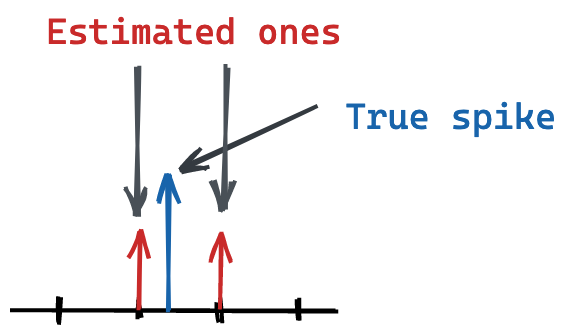
\includegraphics[trim={0 0 0 0},clip,width=\linewidth]{blaster/bodyguard.png}
    \captionof{figure}{%
        Schematics of the \textit{bodyguard effect} affecting on-grid approaches.
    }
    \label{fig:blaster:bodyguard}
}
\begin{itemize}
    \item \textit{Basis mismatch}:
    As explained in~\cref{subsec:estimation:bce}, the filter are not sparse in practice due to the \textit{basis mismatch}.
    This implies that the true peaks of the filter do not necessarily correspond to the true echoes and lead to followings drawbacks.
    \item \textit{The estimation is on-grid}:
    These methods operates fundamentally \textit{on-grid} and return echoes' timings which are integer multiples of the $\Fs$.
    \textit{Bodyguard effect}.
    In addition to affecting the \AER/ performance, on-grid methods may converge slowly to suboptimal solutions.
    In fact, as show in~\cref{fig:blaster:bodyguard}, instead of estimating the peak at its true location, two smaller ``bodyguard'' peaks are estimated around it instead.
    The estimation procedure may stop at this point returning two wrong peaks.
    Having smaller coefficients, this peaks may not be selected by the subsequent peak pickings technique.
    Alternatively, the optimization procedure may continue, alternating tuning the weights of the two ``bodyguards'', without converging to a solution.
    \item \textit{Computational bottleneck}.
    A way to cope with the above limitations is to increase the $\Fs$.
    However this results into a memory and computational bottleneck as several huge (Toeplitz) matrices needs to be built, one for each pair of microphones.
    In addition, this leads the risk that the optimization problem becomes ill-conditioned.
\end{itemize}

\subsection{From cross-relation to LASSO}\label{subsec:blaster:xrel_lasso}
Integrating the sparse penalty and the constraints proposed by~\citeonly{lin2008blind} (See \cref{tab:blaster:sota}) in \cref{eq:blaster:sota},
the \BSNdef/ problem proposed reads
\begin{equation}\label{eq:blaster:bsn}
    \disFilterHat_1, \disFilterHat_2
    =
    \kargmin_{\disFilter_1, \disFilter_2}
    \;
    \tfrac{1}{2}
    \kvvbar{
        \scrT(\disRecordedSignal_1) \disFilter_2
        -
        \scrT(\disRecordedSignal_2) \disFilter_1
    }_2^2
    + \lambda\kvvbar{\bfh}_1
    \;\text{s.t.}\;
    \begin{cases}
        \bfh \geq 0\\
        h_1[0] = 1
    \end{cases}
    .
\end{equation}
This cross-relation based optimization problem can rewritten in the \LASSO/ formulation of~\cref{eq:blaster:lasso} as
\begin{equation*}
    \bfu
    =
    \kargmin_{\bfu}
    \;
    \tfrac{1}{2}
    \kvvbar{ \bfv - \bfB \bfu }_2^2
    + \lambda\kvvbar{\bfu}_1
    \quad\text{s.t.}\quad
    \bfu \geq 0
    ,
\end{equation*}
where
\begin{equation*}
    \bfv = \ttX_2\bfe_1,
    \quad
    \bfu =
    \begin{pmatrix}
        h_1[1:] \\
        h_2
    \end{pmatrix},
    \quad
    \bfA =
    \begin{pmatrix}
        -\ttX_2[:, 1:] & \ttX_1
    \end{pmatrix},
    \quad
    \ttX_i = \scrT(x_i)
    .
\end{equation*}
Here we used the light, yet common, Python notation for indexing the matrices and vectors.

\section{Proposed Approach}
\subsection{Cross-relation in the Fourier domain}
The cross-relation identity~\cref{eq:blaster:cross-relation} ensures that the relation
\begin{equation}
    \idealLowPassFilter
    \ast \contRecordedSignal_1
    \ast  \contFilter_2^\star
    =
    \idealLowPassFilter
    \ast \contRecordedSignal_2
    \ast  \contFilter_1^\star
\end{equation}
holds even during the introducted measurement process, hence
\begin{equation}
    \label{eq:blaster:cross-relation-identity-fourier}
    \fourierTrans(\idealLowPassFilter\ast\contRecordedSignal_1) \cdot \fourierTrans \contFilter_2^\star
    =
    \fourierTrans(\idealLowPassFilter\ast\contRecordedSignal_2) \cdot \fourierTrans \contFilter_1^\star
\end{equation}
where $\fourierTrans$ denotes the \FTdef/ described in~\cref{sec:processing:ft}
\\In contrast with \SIMO/-\BCE/ methods that operates in the time domain, here we propose to use~\cref{eq:blaster:cross-relation-identity-fourier} in a penalized least-square problem.
Such a formulation in the Fourier domain may even be considered as more convenient since the convolution operator is no longer involved.
While the \FT/ of $\contFilter_i^\star$ can be expressed in closed-form (see~\cref{eq:blaster:closed-form-TF-dirac-N} below), the \FT/ of $\idealLowPassFilter\ast\contRecordedSignal_i$ is not available due to the measurement process.
To circumvent this issue, following approximation detailed in~\cref{subsec:processing:ftapprox}, we consider the \DFTdef/ of the $\contRecordedSignal_i$:
\begin{equation}
    \label{eq:blaster:approx-TF}
    \fourierTrans(\idealLowPassFilter\ast\contRecordedSignal_i)
    %(\tfrac{f}{F_s})
    \kparen{\tfrac{k}{2N}F_s}
    \approx
    X_i[k]
\end{equation}
for all integers  $k \in \{0, \ldots, N\}$, where
\begin{equation}
    \label{eq:blaster:dft-Xi}
    \RecordedSignalDFT_i[k] = \sum_{n=0}^{2N-1}
    \disRecordedSignal_i[n]
    \cste^{-\csti2\pi \tfrac{kn}{2N}}
\end{equation}
is the \DFT/ of the real vector $\contRecordedSignal_i$ as defined in~\cref{ch:processing:dft} for positive frequencies only.

\mynewline
Denoting $\paramVec{\tau}$ the following parametric vector of complex exponential
\begin{equation}
    \label{eq:blaster:closed-form-TF-dirac-N}
    \paramVec{\tau} \eqdef
    \left(\cste^{-\csti2\pi\tfrac{k}{2N}F_s \tau}\right)_{0 \leq k \leq N}
    \in\bbC^{N+1}
    ,
\end{equation}
equation the Fourier-domain cross-relation of~\cref{eq:blaster:cross-relation-identity-fourier} evaluated at $f = \frac{k}{2N}F_s$ where $k \in \{0,\ldots, N\}$
reads

\begin{equation}
    \label{eq:blaster:cross-relation-approx}
    \sum_{r=0}^{R_2-1} \alpha_2^{(r)} \RecordedSignalDFT_1 \odot \paramVec{\tau_{2}^{(r)}}
    =
    \sum_{r=0}^{R_1-1} \alpha_1^{(r)} \RecordedSignalDFT_2 \odot \paramVec{\tau_{1}^{(r)}}
\end{equation}
where $\odot$ denotes the component-wise Hadamard product.

\subsection{Echo localization with continuous dictionaries}
By interpreting the \FT/ of a Dirac as a parametric \textit{atom}, we propose to cast the problem of \RIR/ estimation into the framework of \CDdef/.
To this aim, let us define the so-called \emph{parameter set}
\begin{equation}
    \label{eq:blaster:parameter-set}
    \Theta \eqdef \kintervcc{0}{T} \times \kbrace{1, 2}
\end{equation}
where $T$ is the length (in time) of the filter.
Then, the two desired filters  $\contFilter_1^\star,\contFilter_2^\star$ given by~\cref{eq:blaster:def_filter_star} can be uniquely\sidenote{
    Uniqueness is ensured as soon as we impose $\alpha_{i}^{(r)}>0$ $\forall i,r$.
} represented by the following discrete measure over $\Theta$
\begin{equation}
    \label{eq:blaster:representation_filter_measure}
    \mu^\star = \sum_{i=1}^{2} \sum_{r=0}^{R_{i}-1} \alpha_{i}^{(r)} \delta_{(\tau_{i}^{(r)}, i)}.
\end{equation}
where $\delta_{(\tau_{i}^{(r)}, i)}$ denotes the Dirac measure which is different from the Dirac function used when modeling the \RIRs/.
The need of defining a measure over the parameter set $\Theta$ makes easier the parametrization of the problem in the context of \CD/.
For instance, it is possible to define standard operation over measure used in algorithms to solve the such problems.
\\Moreover, the rationale behind~\cref{eq:blaster:parameter-set} and~\cref{eq:blaster:representation_filter_measure} is as follows.
A couple of filters is now represented by a single stream of Diracs, where we have considered an augmented variable $i$ indicating to which filter the spike belongs.
For instance, a Dirac at $(\tau, 1)$ indicates that the first filter contains a Dirac at $\tau$.

\mynewline
The set $\posDisRadonMeasure$ of all unsigned and discrete Radon measures over $\Theta$ (\ie/, the set of all couples of  filters) is equipped with the total-variation norm (TV-norm) $\normTV{\mu}$
\sidenote{See~\citeonly{rudin1987real} for a rigorous construction of measures set and the TV-norm.}.
We now define the \emph{linear} observation operator $\kfuncdef{\opObs}{\posDisRadonMeasure}{\bbC^{N+1}}$, which is such that
\begin{equation}
    \opObs\delta_{(\tau, i)}
    =
    \begin{cases}
        - \RecordedSignalDFT_1 \odot \paramVec{\tau}  &\text{ if } i=1 \\
        + \RecordedSignalDFT_2 \odot \paramVec{\tau}  &\text{ if } i=2.
    \end{cases}
    \qquad \forall(\tau,i)\in\Theta.
\end{equation}

\mynewline
Therefore, by the linearity of the observation operator $\opObs$, the relation~\cref{eq:blaster:cross-relation-approx} can be rewritten as
\begin{equation}
    \label{eq:blaster:cross-relation-measure}
    \opObs\mu^\star = \zeroVect_{N+1}
    ,
\end{equation}
where $\zeroVect_{N+1}$ is a $N+1$-length vector of zeros.
\\Before continuing our exposition, we note that the anchor constraint can be written in a more convenient way.
Indeed, the constraint $\mu(\{(0, 1)\})=1$ ensures the existence of a Dirac at $0$ in the filter $1$.
Then, the targeted filter reads
\begin{equation}
    \mu^\star = \delta_{(0, 1)} + \bar{\mu}^\star
\end{equation}
where $\bar{\mu}^\star$ is a (finite) discrete measure verifying  $\bar{\mu}^\star\kparen{\{(0, 1)\}} = 0$.
\\Denoting $y\eqdef-\opObs\delta_{(0, 1)}\in\bbC^{N+1}$, the relation~\cref{eq:blaster:cross-relation-measure} becomes
\begin{equation}
    \label{eq:blaster:cross-relation-measure-and-obs}
    \opObs\bar{\mu}^\star = y
    .
\end{equation}
For the sake of clarity, we use these conventions hereafter and omit the tilde.
Now, following~\citeonly{de2012exact,candes2014towards}, one can expect to recover the desired filter $\mu^\star$ by solving
\begin{equation}
    \stepcounter{equation}
    \tag{\theequation-$\calP^0{\text{\texttt{TV}}}$}
    \label{eq:blaster:TV-BP}
    \widehat{\mu}
    =
    \kargmin_{\posDisRadonMeasure}
    \;
    \normTV{
        \mu
    }
    \quad
    \text{s.t.}
    \quad
    \begin{cases}
        \opObs\mu
        = y \\
        \mu(\{(0, 1)\}) = 0.
    \end{cases}
\end{equation}
Note that~\eqref{eq:blaster:TV-BP} has to be interpreted as a natural extension of the well-known \emph{basis pursuit} problem to the continuous setting.
Indeed, for \emph{any} finite discrete measure $\mu = \sum_{r=0}^{R-1} \alpha^{(r)}\delta_{(\tau^{(r)}, i^{(r)})}$, the TV-norm of $\mu$ returns to the $\ell_1$-norm of the coefficients, \ie/, $\kvvbar{\mu}_{TV} = \sum_{\idxEch=0}^{\numEchs-1} \kvbar{\alpha^{(r)}}$.

\mynewline
Finally,~\cref{eq:blaster:cross-relation-measure-and-obs} can be exploited to take into account noise during the measurement process (\ie/,  $n_i\neq0$ in~\cref{eq:blaster:recordedSignal}), as well as approximation errors  (see~\cref{eq:blaster:approx-TF}-\cref{eq:blaster:cross-relation-approx}).
In that case, the first equality constraint in~\eqref{eq:blaster:TV-BP} is relaxed, leading to the so-called \BLASSO/ problem
\begin{equation}
    \stepcounter{equation}
    \tag{\theequation-$\calP^\lambda_{\text{\texttt{TV}}}$}
    \label{eq:blaster:TV-BLASSO}
    \begin{split}
    \widehat{\mu}
    =
    \kargmin_{\mu \in\posDisRadonMeasure}
    \;
    \tfrac{1}{2} \kvvbar{
        y - \opObs\mu
    }_2^2
    +
    \lambda\normTV{
        \mu
    }
    \quad
    \text{s.t.}
    \quad
    \mu(\{(0, 1)\}) = 0
    .
    \end{split}
\end{equation}
We emphasize that although continuous Radon measures may potentially be admissible, the minimizers of~\cref{eq:blaster:TV-BLASSO} are \emph{guaranteed} to be streams of Dirac\textit{s}~\citeonly[Theorem~4.2]{bredies2020sparsity}.
In addition, although problem~\cref{eq:blaster:TV-BLASSO} seems to depend on some regularization parameter $\lambda$, we describe in~\cref{sec:blaster:lambda} a procedure to automatically tune it to recover a desired number of spikes.
Finally, note that problem~\cref{eq:blaster:TV-BLASSO} is convex with linear constraints over the parameter set $\Theta$.
Therefore, theoretically, the problem can be solved exactly.
However, in practice, optimization over space of measures, still complicated because many steps can only be done up to a prescribed precision.
% 1) you define atome function (14) without the dirac measure
% ex: a: tau -> a(tau)
% 2) you define the desired filter as \sum_{c_{i, r}} a(\tau_{i, r})
% 3) The How?
% 4) existing work of antoine and Helena
% fix the number of echoes
% say c_1... \tau_1... = \argmin someting
% frawback complicated, non convex and so
% 5) idea: rephrease is a convex formulation
% -> convenient framework is set of measurexs of theta
% Convex in the measure
% theoretically, we have algorithm to solve the  problkem exactly
% But in practice, optimization over space of measures, still complicated
% because many steps can only be done up to a prescribedf precision
% (unkike classical convex optimization)
% step 7 and 15

\subsection{From LASSO to BLASSO}
In order to better understand the proposed approach based on the \BLASSO/ algorithm, we can present it in light of the \LASSO/ formulation.
\begin{gather*}
    \kargmin_\bfu \tfrac{1}{2} \kvvbar{\bfv - \bfA \bfu}_2^2 + \lambda \kvvbar{\bfu}_1 \;\text{s.t.}\; \bfu \geq 0\\
    \downarrow\\
    \kargmin_\bfu \tfrac{1}{2} \kvvbar{y - \opObs\mu}_2^2 + \lambda \normTV{\mu} \;\text{s.t.}\; \mu \in\posDisRadonMeasure\\
\end{gather*}
Now, some parallelism can be envisioned:
\begin{itemize}
    \item\textit{From dictionary to operator}:
    The matrix $\bfA$ is typically referred to as \textit{dictionaries}.
    Then selecting the $l$-th column of the dictionaries, \ie/ $\bfA\bfe_l$, means selecting an echo at location $l$-th \wrt/ the vector $\bfu = \bfh[1:]$.
    In the context of \CD/, the dictionary is translated into the operator $\opObs$ thanks to the closed-from of the atom based on the Fourier theory.
    Therefore, $\opObs(\delta_\tau)$ can be seen as the selection of an echo at location $\tau \in [0, T]$~ms.
    \item\textit{Solution}:
    The \LASSO/-like approach promotes a solution $\bfu = \bfh[1:]$ which is sparse and non-negative vector. The last one, ensured by the non-negativity constraint.
    In the \BLASSO/, this is translated assuming the spike measure assumed for the channels, namely, $\mu = \sum_r \alpha^{(r) \delta(t - \tau^{(r)})}$.
    \item\textit{Sparsity}: while in the initial case, the sparsity is enforced by the $\ell_1$-norm, in the second case it is pursued with the TV-norm.
    \item\textit{Solver}: the former optimization problem can be solved with standard \LASSO/ solvers, while for the latter a gradient-descent algorithm is used.
\end{itemize}

\marginpar{
    \vspace{-15\baselineskip}
    \centering
    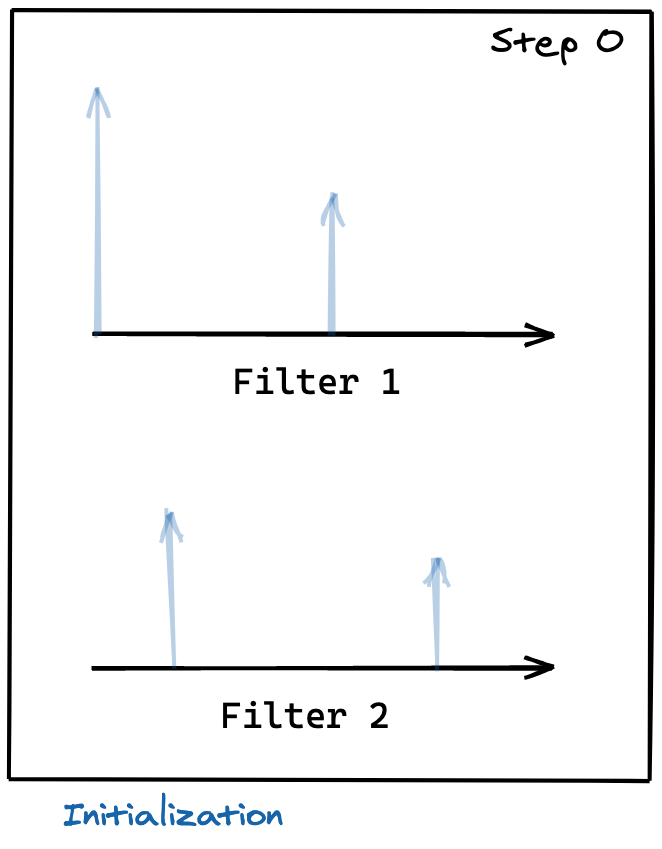
\includegraphics[width=0.5\linewidth]{blaster/echo0.png}\\
    $\downarrow$\\
    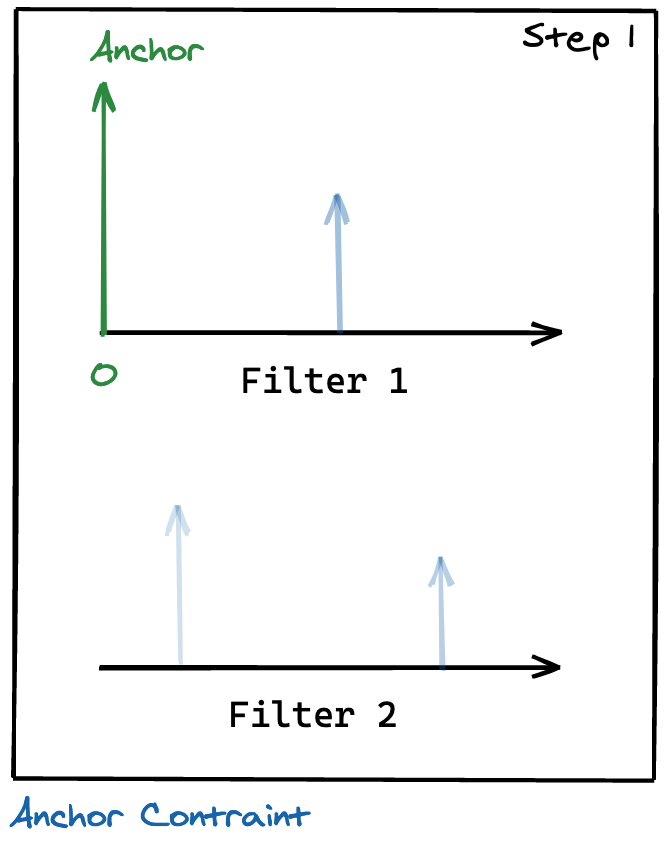
\includegraphics[width=0.5\linewidth]{blaster/echo1.png}\\
    $\downarrow$\\
    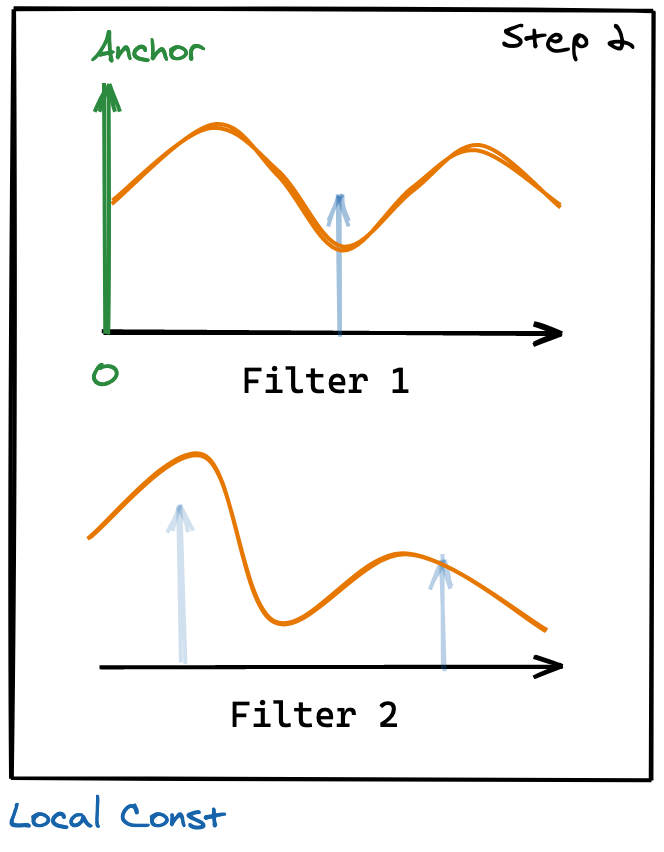
\includegraphics[width=0.5\linewidth]{blaster/echo2.png}\\
    $\downarrow$\\
    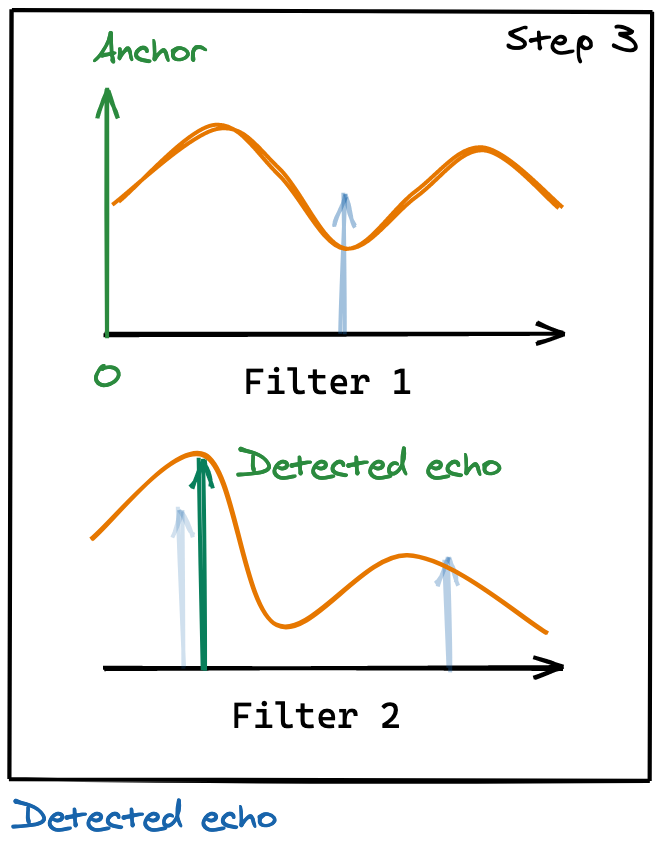
\includegraphics[width=0.5\linewidth]{blaster/echo3.png}\\
    $\downarrow$\\
    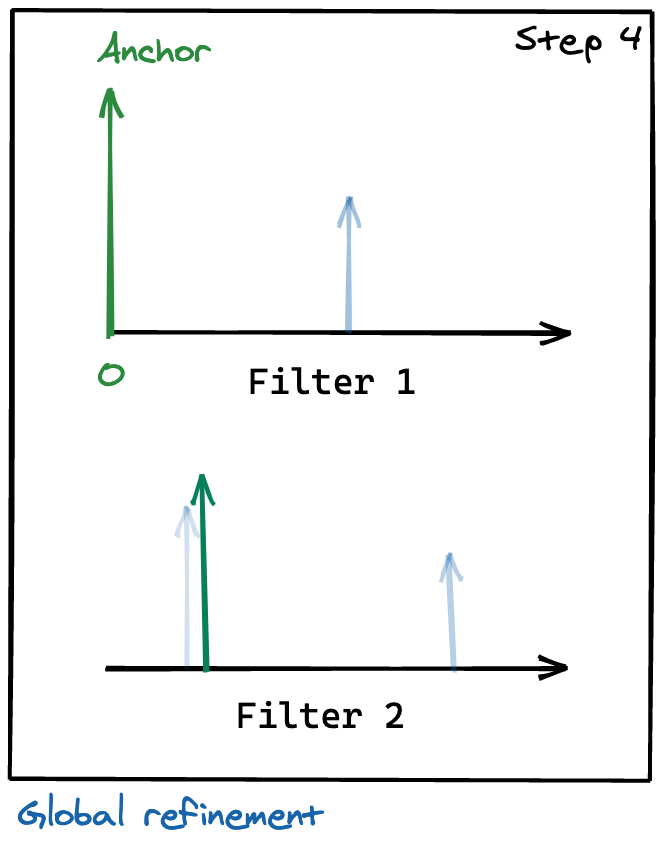
\includegraphics[width=0.5\linewidth]{blaster/echo4.png}\\
    $\downarrow$\\
    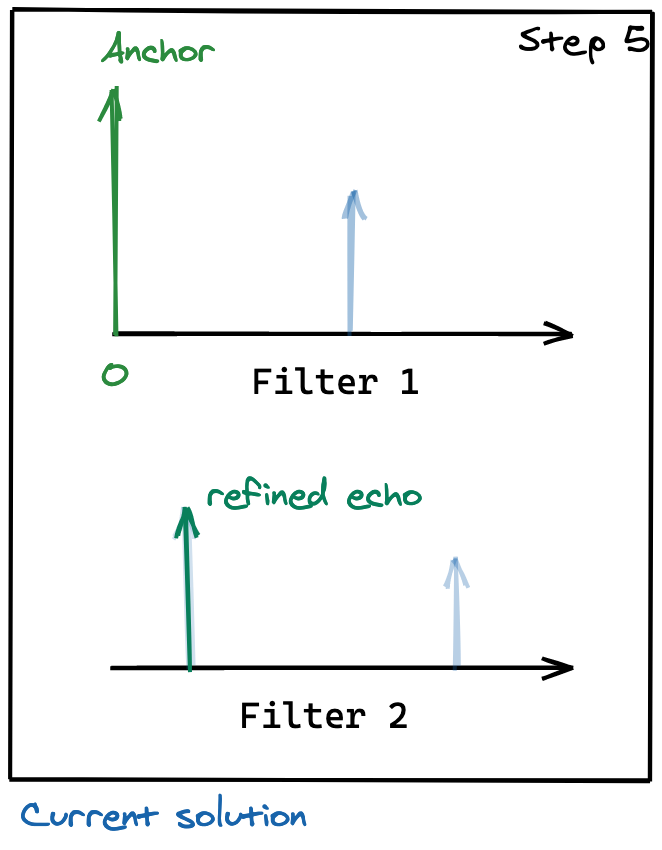
\includegraphics[width=0.5\linewidth]{blaster/echo5.png}
    \captionof{figure}{
        Illustration of the sliding Frank-Wolfe algorithm proposed in~\citeonly{denoyelle2019sliding} in \BLASTER/.
    }
    \label{fig:blaster:sfw}

}

\subsection{The resulting algorithm}
The algorithm used to solve~\cref{eq:blaster:TV-BLASSO} is an instance the sliding Frank-Wolfe algorithm proposed in~\citeonly{denoyelle2019sliding} to solve~\cref{eq:blaster:TV-BLASSO}.
Detailed descriptions of the steps of the algorithm are given in~\cref{ap:blaster}.
In a nutshell, the algorithm iterative over the following steps until a condition on the cost function is met.
\begin{enumerate}
    \item \textit{Anchor constrain.}
    At first the anchor constraint in added arbitrarily on one of the two filters. This is used to initialize the two filters;
    \item \textit{\textit{Local} cost based on Cross-relation}
    For both the filters, a local cost-function derived from the cross-relation for both the filters is computed;
    At this step either the initialization or previously found solution are used;
    \item \textit{Find the maximizer}
    a new candidate echo's location is found as maximizer among the two local cost functions of the previous step;
    \item \textit{Update the amplitudes}
    By solving a non-negative \LASSO/ problem, all the echo's amplitude coefficients estimated until this point are updated;
    \item \textit{Joint refinement}
    The position and the coefficient of the current solution are jointly refined to ease numeric resolution using the original cost function.
    \item \textit{Current solution and repeat}
    The algorithm stops as soon as an iterate satisfies the first order optimality condition associated to the convex problem;
    if not, the algorithm iterates from step 2. using the current solution as input.
\end{enumerate}
These steps are illustrated in~\cref{fig:blaster:sfw}.
% \begin{figure}[h]
%     \begin{fullwidth}
%     \centering
%     \subfloat[echo0][Anchor]{
%         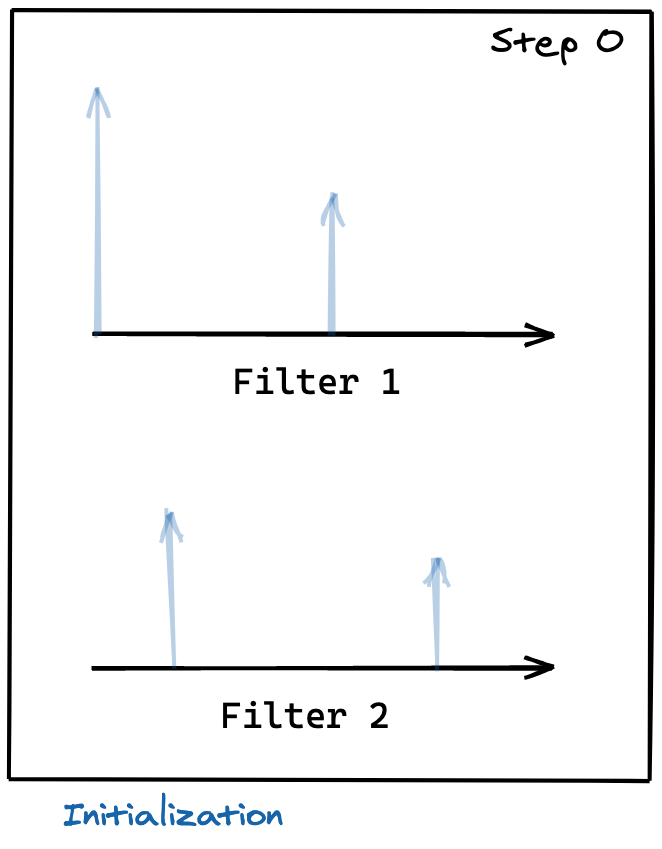
\includegraphics[width=0.13\linewidth]{blaster/echo0.png}
%         \label{fig:blaster:echo0}}
%     \hfill
%     \subfloat[echo1][Local evaluation]{
%         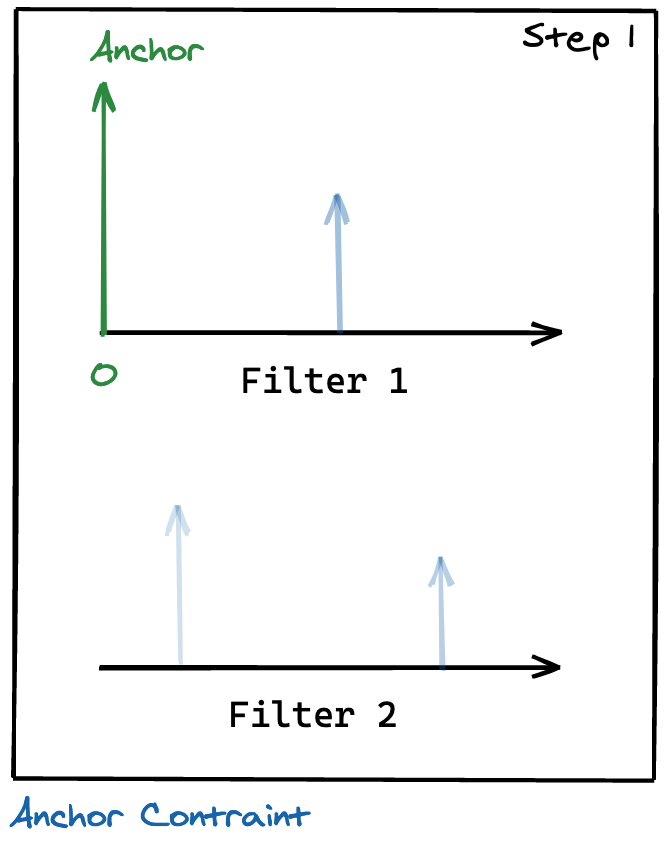
\includegraphics[width=0.13\linewidth]{blaster/echo1.png}
%         \label{fig:blaster:echo1}}
%     \hfill
%     \subfloat[echo2][Maximizer]{
%         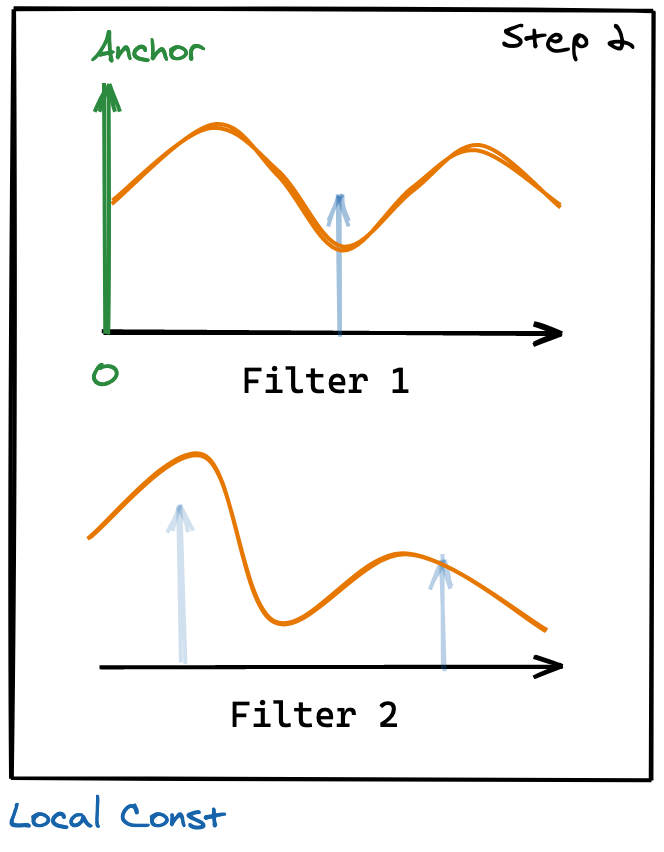
\includegraphics[width=0.13\linewidth]{blaster/echo2.png}
%         \label{fig:blaster:echo2}}
%     \\
%     \subfloat[echo3][Update echoes' amplitudes]{
%         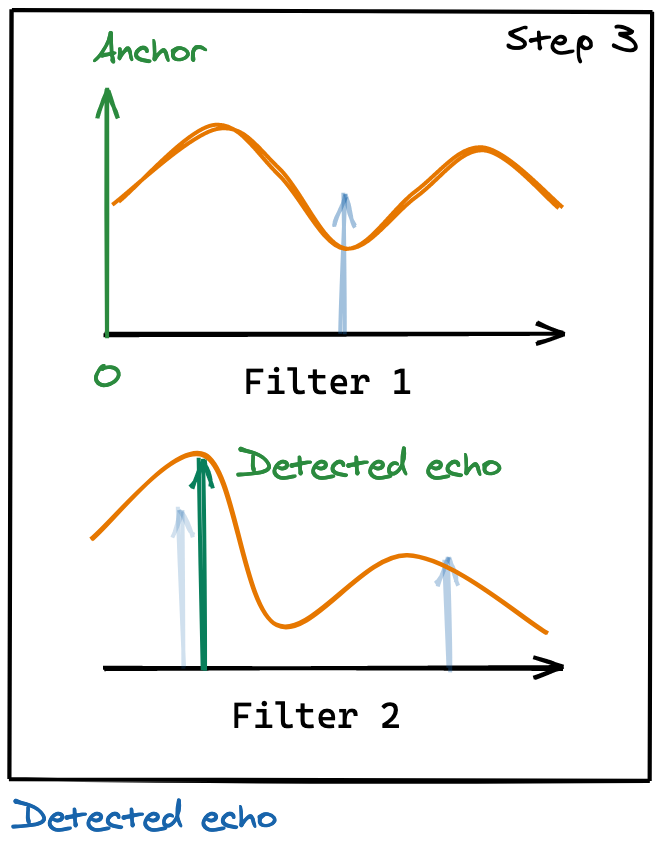
\includegraphics[width=0.13\linewidth]{blaster/echo3.png}
%         \label{fig:blaster:echo3}}
%     \hfill
%     \subfloat[echo4][Joint refinement]{
%         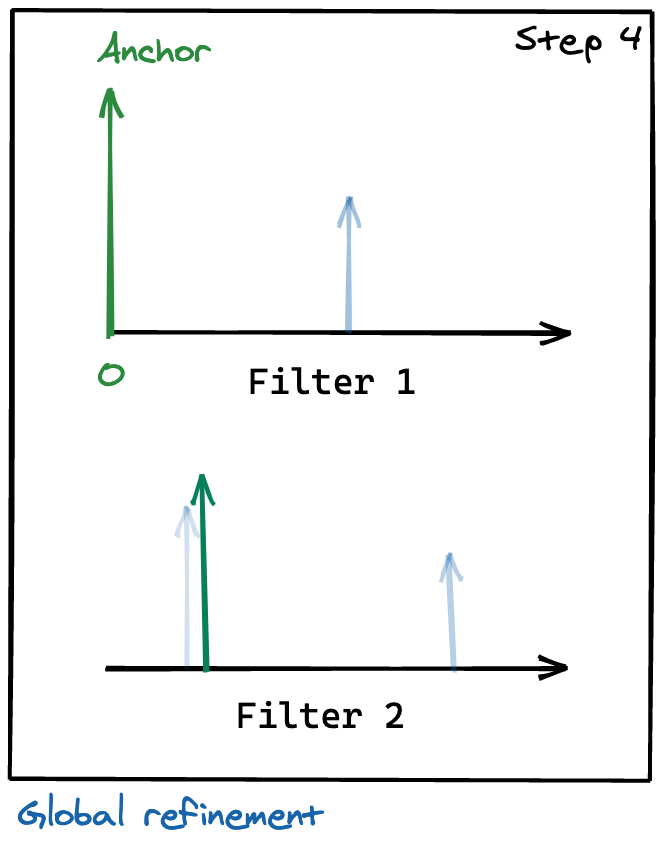
\includegraphics[width=0.13\linewidth]{blaster/echo4.png}
%         \label{fig:blaster:echo4}}
%     \hfill
%     \subfloat[echo5][Current solution]{
%         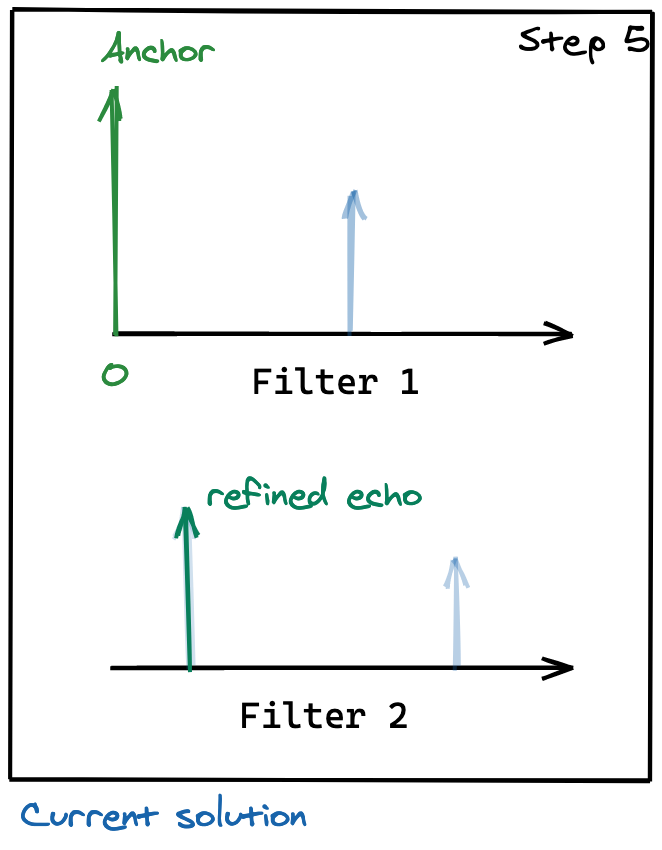
\includegraphics[width=0.13\linewidth]{blaster/echo5.png}
%         \label{fig:blaster:echo5}}
%     \hfill
%     \end{fullwidth}
% \end{figure}

\subsection{Homotopic path for $\lambda$ estimation}\label{sec:blaster:lambda}
Existing works, as well as the proposed one, relies of the regularization $\lambda$ parameter to weight the sparsity penalty.
However, this becomes an hyperparameter that needs to be carefully tuned according to the input data.
Instead, we propose to compute a \textit{path of solutions} to automatically estimate it in~\cref{eq:blaster:TV-BLASSO}.
In the context of sparse optimization this technique is also referred to as \textit{homotopic path}.
More precisely, let $\lambda_{\max}$ be the smallest value of $\lambda$ such that the null measure is the solution to~\cref{eq:blaster:TV-BLASSO}.
It can be shown that $\lambda_{\max}$ is upper bounded by $\max_{\theta\in\Theta} \kvbar{y^\intercal\opObs\delta_\theta}$ (See~\cref{ap:blaster}).
Starting from $z=1$ and the empty filter, we consider a sequential implementation where the solution of~\cref{eq:blaster:TV-BLASSO} is computed for $\lambda^(z)= 10^{-0.05z}\lambda_{\max}$ until the desired number of spikes is found in each channel when incrementing $z$.
For each $\lambda^(z)$, we search for a solution of~\cref{eq:blaster:TV-BLASSO} with the solution obtained for $\lambda^{(z-1)}$ as a warm start.

\section{Experiments}\label{sec:blaster:exp}
The proposed method (\BLASTER/) is compared against the non-negative $\ell_1$-norm method (\algoBsn) of~\citeonly{lin2007blind} and the iterative $\ell_1$-norm approach (\algoCrocco) described in~\citeonly{crocco2016estimation}.
The problem is formulated as estimating the time location of the first $\numEchs=7$ strongest components of the RIRs for 2 microphones listening to a single sound source in a shoebox room. It corresponds to the challenging task of estimating first-order early reflections.
The robustness of the methods is tested against different level of noise (SNR) and reverberation time (\RT{}).

\mynewline
The quality of the AER estimation is assessed in terms of precision\sidenote{
    Since only $K$ time locations are considered in both the ground truth and the estimation, precision and recall are equal.}
in percentage as in the literature of onset detection~\citeonly{bock2012evaluating} and the \RMSEtxt/ in samples.
Both metrics evaluate only the \textit{matched} peaks, where a \textit{match} is defined as being within a small window $\thr$ of a reference delay.
These two metrics are similar to the ones used in~\citeonly{crocco2015room}.

\mynewline
For this purpose we created three synthetic datasets of $1000$ observations each, which are summarized in Table~\cref{tab:blaster:datasets}.
\begin{table}[ht]
    \begin{sidecaption}[]{
        Summary of the dataset used for evaluation. \epsdice[black]{3} and \epsdice{5} stands for randomly sampled from a continuous and discrete set of values respectively
    }[tab:blaster:datasets]
    \centering
    \small
    \begin{tabular}[t]{lccc}
    \toprule
    Dataset      & Signals & SNR [dB] &  $\RT{}$ [s]\\
    \midrule
    \dsetValid     & broadband noise & \epsdice[black]{3} & \epsdice[black]{3}\\
    \dsetSNR       & broadband noise, speech  &\epsdice{5} & $400$ ms\\
    \dsetRT        & broadband noise, speech  &$20$ dB  & \epsdice{5}\\
    \bottomrule
\end{tabular}
    \end{sidecaption}
\end{table}
\\\dsetValid{} is used for tuning the hyperparameter $\lambda$ and the peak-picking parameters for \algoCrocco{} and \algoBsn{} using \RT{} and SNR randomly drawn from $\mathcal{U}[0, 1]$ (sec) and $\mathcal{U}[0, 20]$ (dB) respectively; \dsetSNR{} features SNR value uniformly sampled in $[0, 6, 14, 20, \infty]$ while the \RT{} is kept fixed to $400$ ms; akin the \dsetRT{} is built sampling \RT{} value uniformly in $[200, 400, 600, 800, 1000]$ ms keeping SNR fix to 20 dB.
Moreover, while for \dsetValid{} broadband signals (white noise) are used as the source, for \dsetSNR{} and \dsetRT{} speech utterances from the TIMIT dataset are also included.
The signal duration is kept fixed to 1 s with sampling frequency $\Fs = 16$ kHz.
For a given \RT{} value and room with random dimensions, a unique absorption coefficient is assigned to all surfaces based on the Sabine's formula.
Then, the two microphones and the source are randomly positioned inside the room.
The parameters of such audio scene are then passed as input to the \pyroomacoustics{} simulator~\citeonly{scheibler2018pyroomacoustics}, which returns the corresponding \RIRs/ as well as the \textit{off-grid} echo delays and attenuation coefficients computed with the \ISMdef/~\citeonly{allen1979image}.
Note that when generating the data, no samples have been pruned to match any minimal separation condition.
To generate the microphone signals, an over-sampled version of the source signal is convolved with ideal \RIRs/ at high frequency ($\Fs=1024$ kHz) made up of on-grid Dirac\textit{s}. The results are later resampled to meet the original $\Fs$ and Gaussian white noise is added to meet the given SNR value.

\begin{figure}[ht]
    \centering
    \begin{fullwidth}
        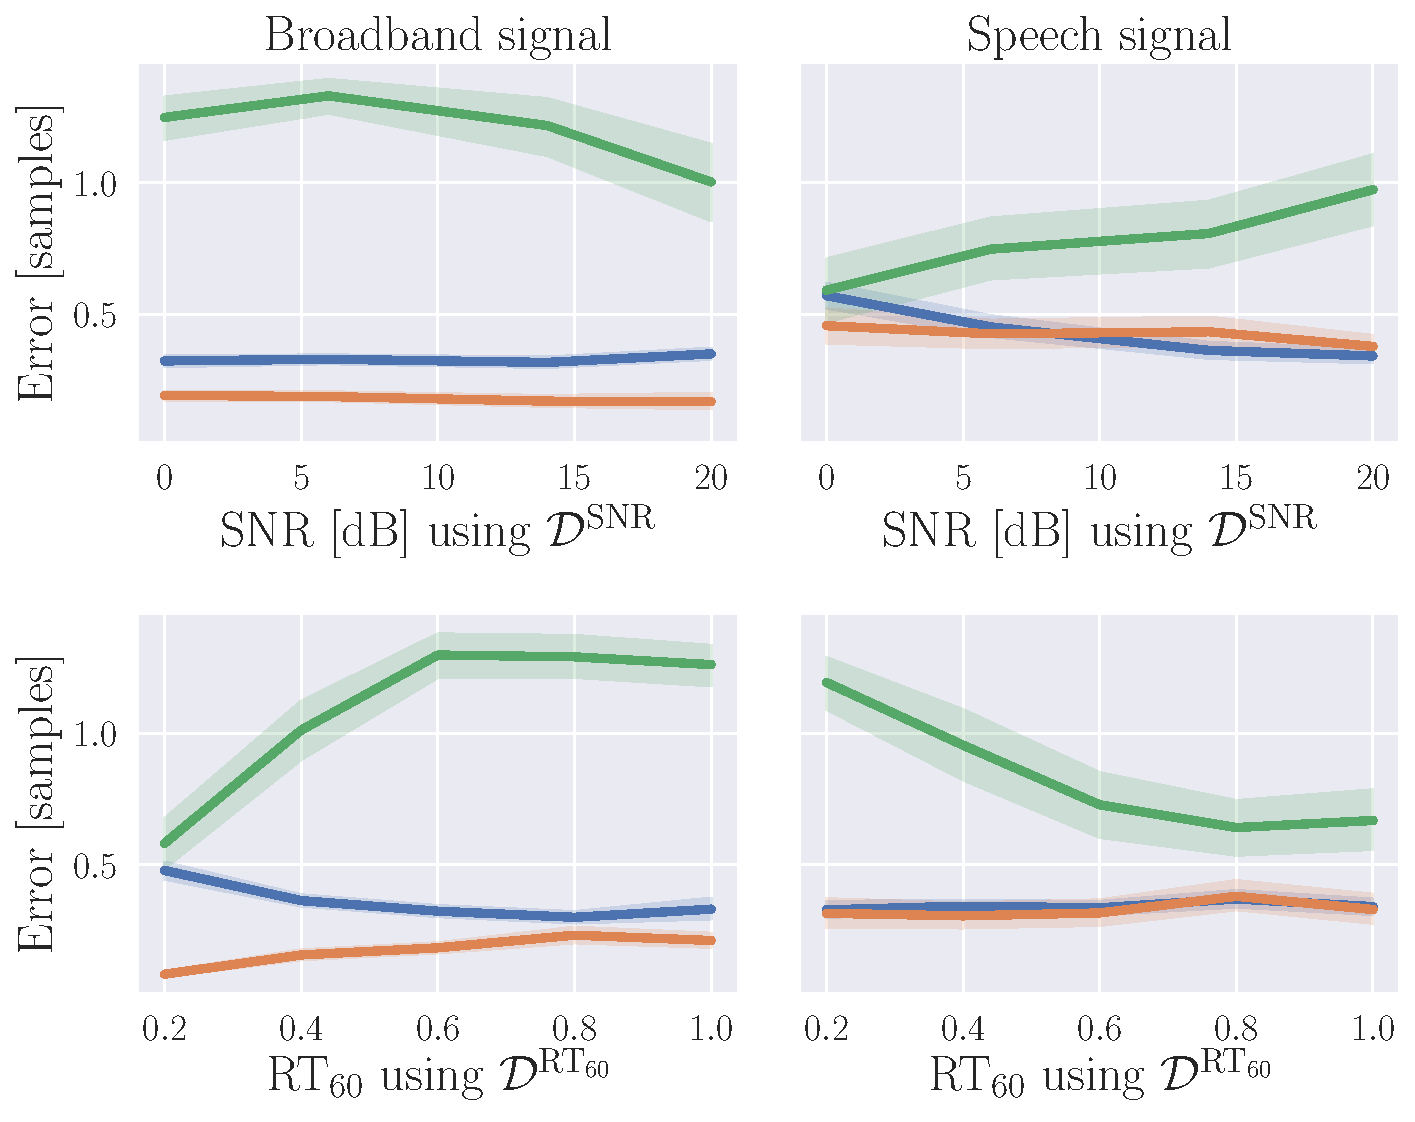
\includegraphics[width=.49\textwidth]{figures/blaster/e_k-7_thr-2_bns_crocco_blaster.pdf}
        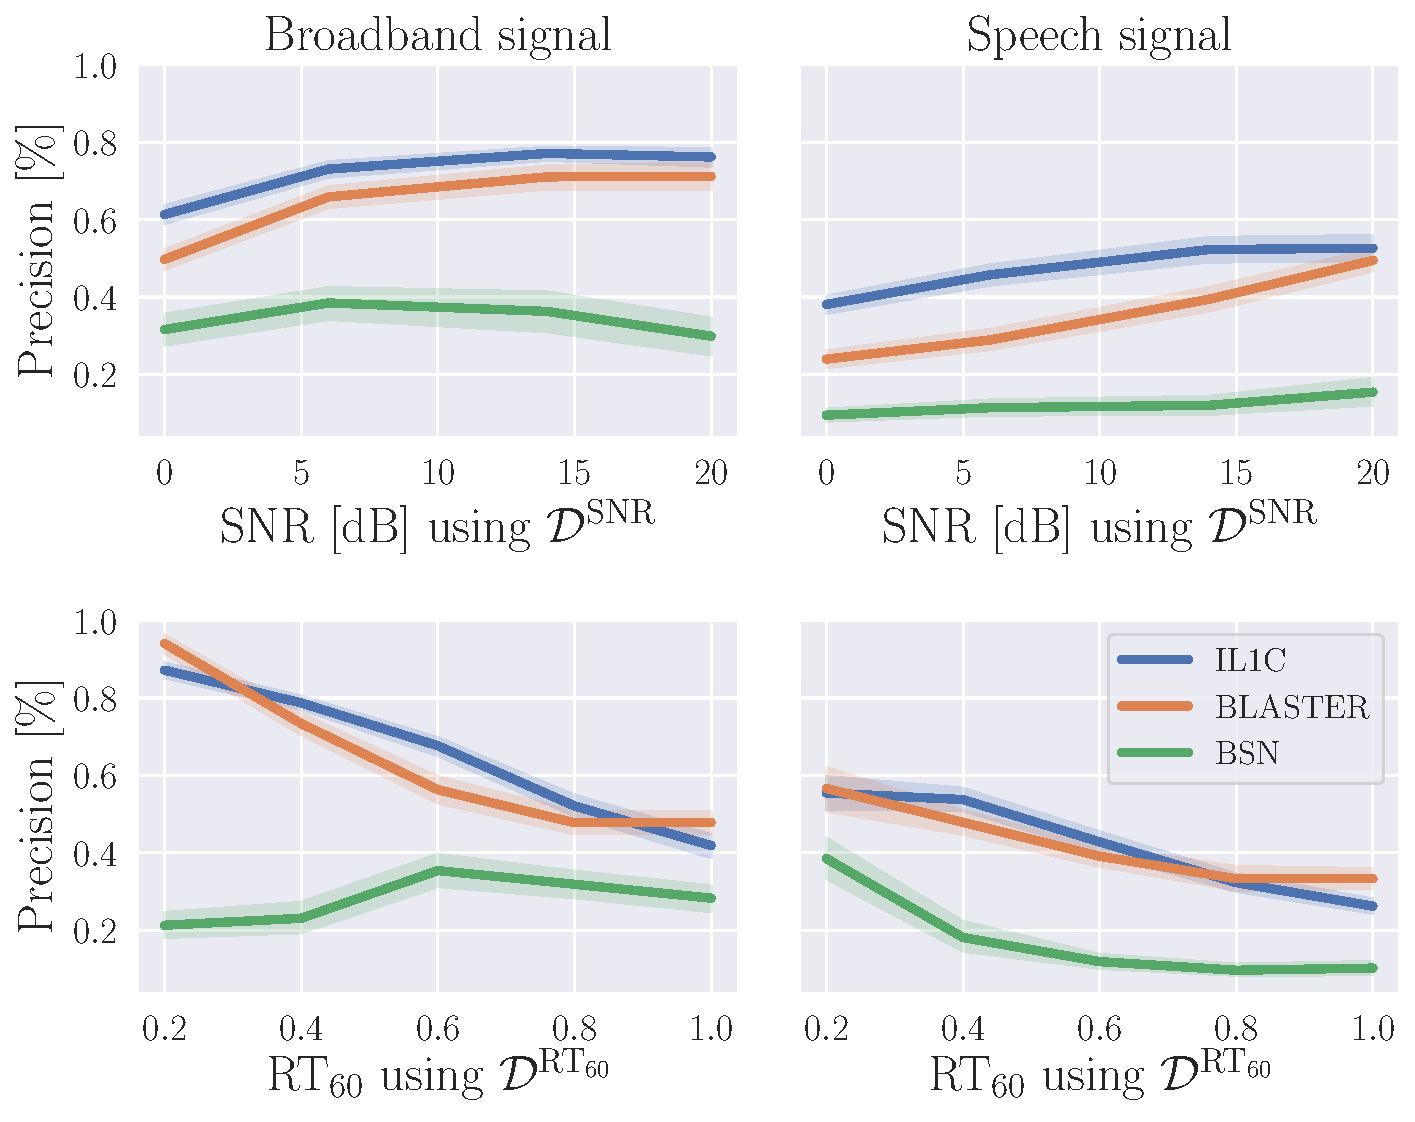
\includegraphics[width=.49\textwidth]{figures/blaster/p_k-7_thr-2_bns_crocco_blaster.pdf}
        \caption{%
            \label{fig:error_precision_snr_rt}
            Line plot with error bands for error (left) and precision (right) versus SNR level (top) and \RT{} level (bottom) using broadband and speech signals for the task of recovering $\numEchs=7$ echoes. A threshold of $\tau_{\textrm{max}}=2$ samples is used to compute the precision.
        }

    \end{fullwidth}
\end{figure}

\begin{table}[ht]
    \begin{sidecaption}[]{
        Precision for different threshold $\thr$ in samples for the recovery of $R = 2$ and $7$ echoes, \RT{} = $200$ ms and SNR = 20 dB.
    }[tab:error_precision_thr]
    \centering
    \footnotesize
    %\begin{table}[t]
    {
        \centering
        \begin{tabular}{lccccc|ccccc}
        \toprule
               & \multicolumn{10}{c}{Precision [\%]}	\\
               \cline{2-11}
               & \multicolumn{5}{c|}{R = 2 echoes} & \multicolumn{5}{c}{R = 7 echoes} \\
               %
               \hline
               %
    $\thr$ & $0.5$ & $1$ & $2$ & $3$ & $10$ & $0.5$ & $1$ & $2$ & $3$ & $10$ \\ \hline
    BSN &  8 &           9 &          27 &          46 &           62 &           5 &           8 &          38 &          54 &  {73}  \\
    IL1C &           51 &          55 &          55 &          56 &           58 &          42 &          53 &          55 &          56 &         58 \\
    BLASTER & \textbf{68}  & \textbf{73}  & \textbf{74}  & \textbf{75}  & \textbf{75}   &{46}  &          53 &  {56}& {57} &         61 \\
    \bottomrule
    \end{tabular}
    }
    %\end{table*}


    % %\begin{table*}[t]
    % {
    %     \centering
    %     \scriptsize
    %     \begin{tabular}{lcccccccccc|ccccc|ccccc}
    %     \toprule
    %            & \multicolumn{10}{c|}{Error [samples]}                                                                                               & \multicolumn{10}{c}{Precision [\%]}                                                                           \\ \cline{2-21}
    %            & \multicolumn{5}{c|}{K = 2 echoes}                                           & \multicolumn{5}{c|}{K = 7 echoes}                     & \multicolumn{5}{c|}{K = 2 echoes}                     & \multicolumn{5}{c}{K = 7 echoes}                     \\ \hline
    % $\thr$ & $0.5$ & $1$ & $2$ & $3$ & \multicolumn{1}{c|}{$10$} & $0.5$ & $1$ & $2$ & $3$ & $10$ & $0.5$ & $1$ & $2$ & $3$ & $10$ & $0.5$ & $1$ & $2$ & $3$ & $10$ \\ \hline
    % \algoBsn &  \textbf{0.01} &\textbf{0.05}&        1.07 &        1.53 &\multicolumn{1}{c|}{2.85}         &\textbf{0.05}&        0.24 &        1.19 &        1.53 &         3.09 &           8 &           9 &          27 &          46 &           62 &           5 &           8 &          38 &          54 & \textbf{73}  \\
    % \algoCrocco &        0.20 &        0.23 &        0.24 &        0.26 &\multicolumn{1}{c|}{0.40}         &        0.20 &        0.28 &        0.33 &\textbf{0.37}&\textbf{0.83} &          51 &          55 &          55 &          56 &           58 &          42 &          53 &          55 &          56 &         58 \\
    % \algoBraire &        0.06 &        0.10 &\textbf{0.14}&\textbf{0.20}&\multicolumn{1}{c|}{\textbf{0.34}}&        0.13 &\textbf{0.20}&\textbf{0.32}&        0.42 &         1.48 &\textbf{68}  &\textbf{73}  &\textbf{74}  &\textbf{75}  &\textbf{75}   &\textbf{46}  &          53 &  \textbf{56}& \textbf{57} &         61 \\
    % \bottomrule
    % \end{tabular}
    % }
    %\end{table}
    \end{sidecaption}
\end{table}

\begin{figure}[t!]
    \begin{sidecaption}[]{
        Line plots with error bands of precision versus number of echoes $R$ to be retrieved for broadband (left) and speech (right) signals with \RT{} = $400$ ms and SNR = 20 dB.
    }[fig:error_precision_kecho]
    \centering
    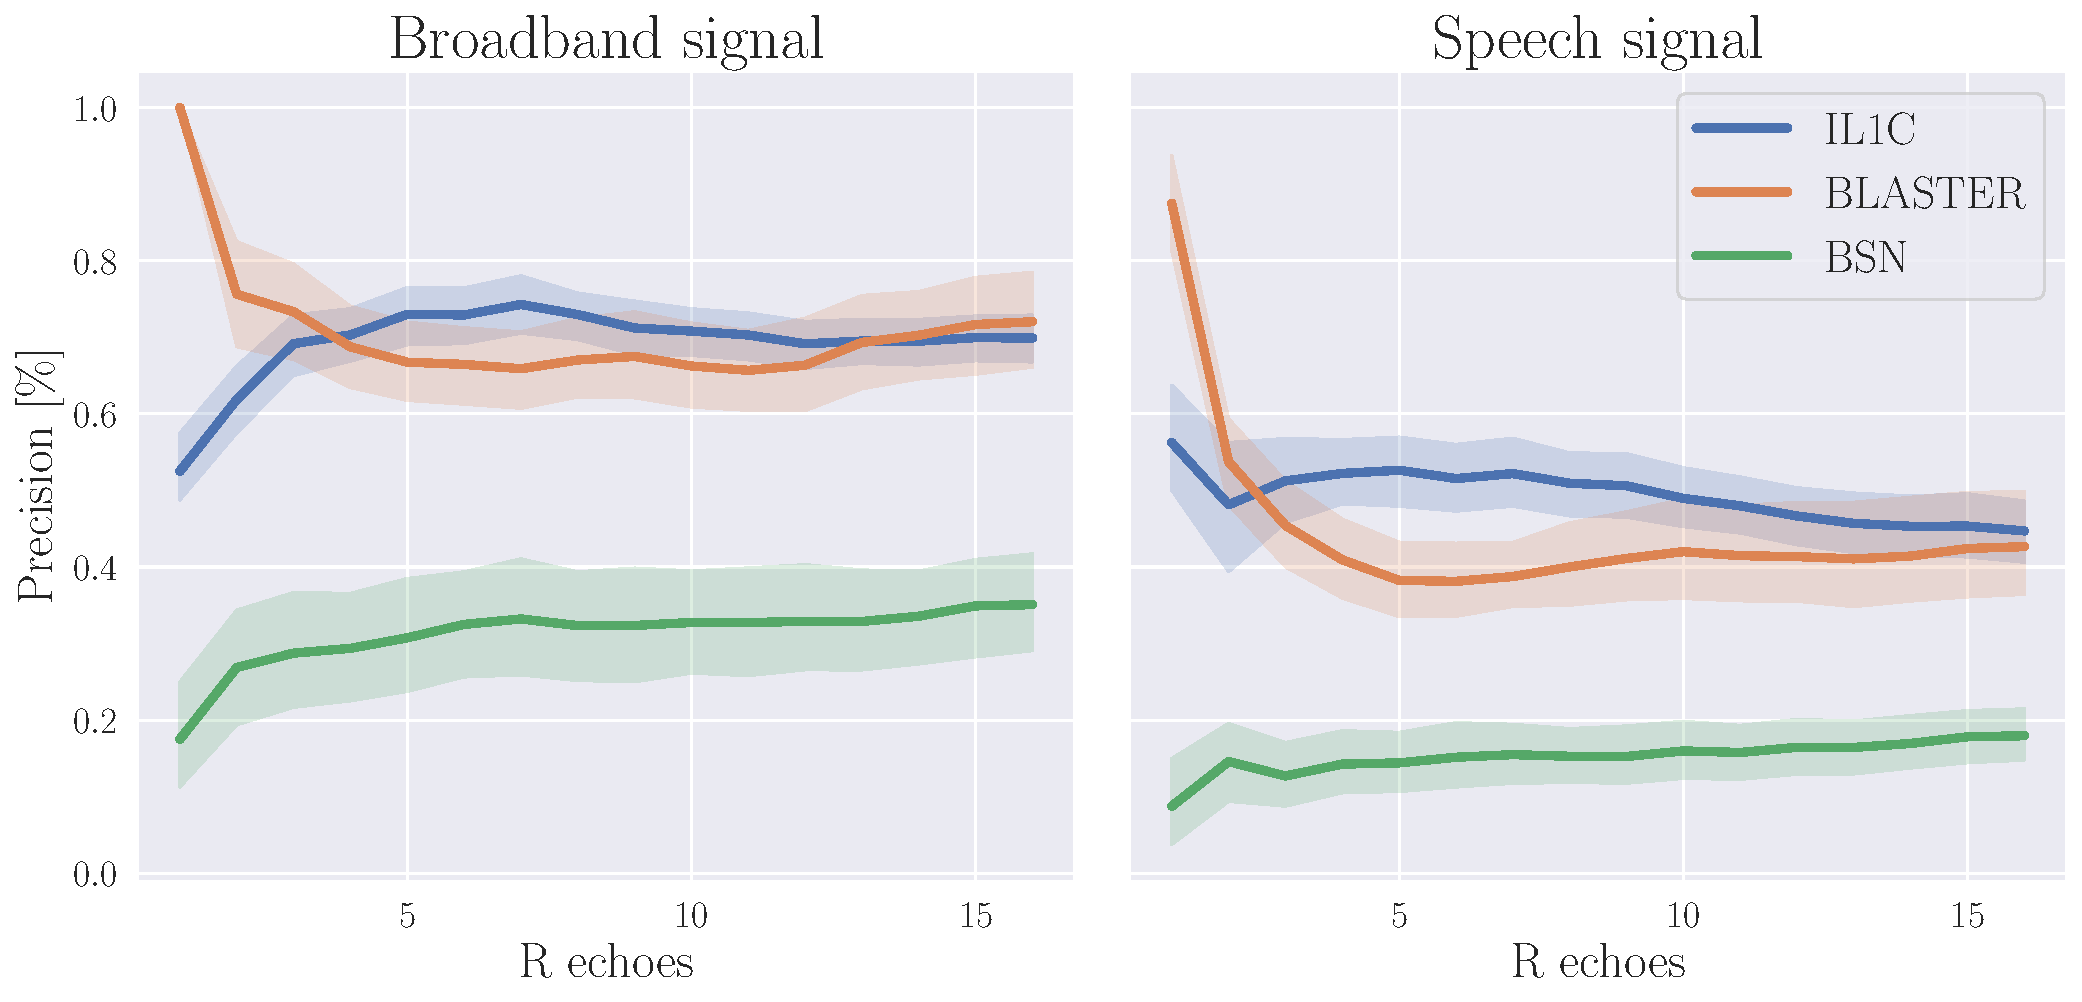
\includegraphics[width=\linewidth]{figures/blaster/p_k-7_thr-2_bns_crocco_blaster-peak_withRechoes.pdf}
    \end{sidecaption}
\end{figure}

\newthought{Quantitative results} are reported in ~\cref{fig:error_precision_snr_rt}, ~\cref{fig:error_precision_kecho} and ~\cref{tab:error_precision_thr}.
Here, for both RMSE and Precision and for both broadband and speech signal, the metrics are displayed against the dataset parameters.
We observe that \algoBsn{} performs worst in all tested conditions, possibly due to its strong reliance on the peak picking step.
For $\numEchs=7$ or higher, \algoBraire{} yields similar or slightly worse performance than \algoCrocco{} for the considered noise and reverberation levels, with decreasing performance for both as these levels increase.
Using speech rather than broadband signals also yields worse results for all methods.
However, the echo timing RMSE is significantly smaller using \algoBraire{} due to its off-grid advantage. We also note that \algoBraire{} significantly outperforms \algoCrocco{} on the task of recovering $\numEchs=2$ echoes. As showed in Tab.~\ref{tab:error_precision_thr}, in mild conditions, up to 68\% of echoes can be retrieved by \algoBraire{} with errors lower than half a sample in that case.
This is promising since the practical advantage of knowing the timing of two echoes per channel has been demonstrated in~\citeonly{di2019mirage,scheibler2018separake}.

\section{Conclusion}
A novel blind, off-grid, multichannel echo retrieval method has been proposed based on the framework of continuous dictionaries.
Comparisons with state-of-the-art approaches on various noise and reverberation conditions show that this method performs best when the number of echoes to retrieve is small.
While some robustness to noise, reverberation, and non-broadband signals is observed, our experiments reveal that room for improvement exists for this challenging and emerging topic.
Future works will include an extension to more than two channels and experiments on real-world data.